\begin{figure*}[t]
\centering
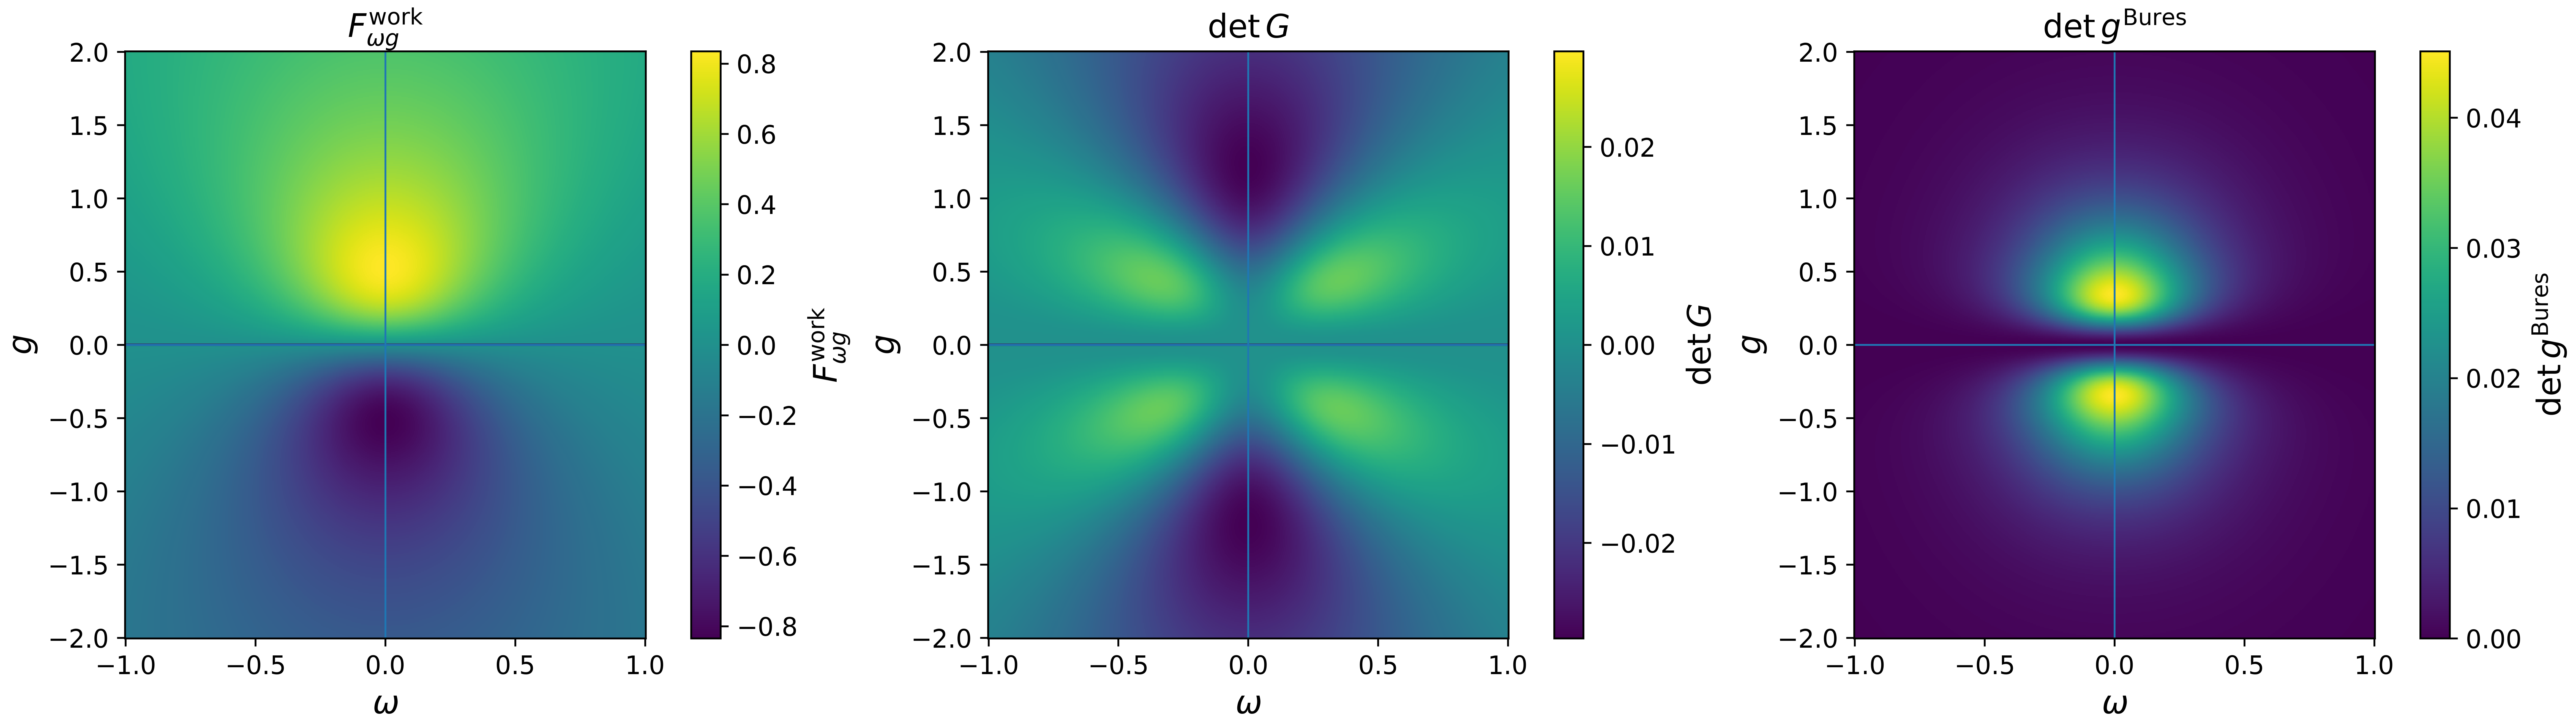
\includegraphics[width=\textwidth]{Figures/Figure1_F_vs_G_vs_g.png}
\caption{
\textbf{Comparison of response geometry and information geometry for a driven open quantum system.}
The three panels display complementary geometric structures
defined over the same two-dimensional control manifold
parameterized by the Hamiltonian frequency $\omega$ and coherent
coupling strength $g$. All quantities are computed from the same
family of nonequilibrium stationary density operators of the
driven qubit model.
(a) Antisymmetric work curvature
$F_{\omega g}^{\rm work}$.
This field governs the geometric contribution to quasistatic
cyclic work and changes sign under reversal of the orientation of
the control cycle. The nodal line separates regions of opposite
geometric orientation and is analogous to the curvature fields
introduced earlier for equilibrium thermodynamic systems.
(b) Determinant of the symmetric response metric,
$\det G$.
This quantity measures the magnitude of the reciprocal component
of the local response tensor and characterizes the local
susceptibility of the nonequilibrium steady state to changes in
the external control parameters. Unlike the antisymmetric
curvature, the response metric is insensitive to the orientation
of parameter-space loops.
(c) Determinant of the Bures metric,
$\det g^{\rm Bures}$.
The Bures metric is an information-geometric measure of the
distinguishability of neighboring stationary density operators
and is proportional to the quantum Fisher information. It
contains no antisymmetric component and therefore cannot describe
geometric work or nonreciprocal response.
Although all three fields are generated from the same family of
stationary states, they exhibit markedly different spatial
organization. The work curvature possesses a signed dipolar
structure associated with nonreciprocal response, the response
metric develops a quadrupolar pattern characteristic of
reciprocal susceptibility, and the Bures metric is localized near
the avoided crossing where neighboring stationary states become
most rapidly distinguishable. Their coexistence demonstrates that
nonequilibrium quantum systems possess multiple, complementary
geometric structures. Response geometry and information geometry
are therefore related through the common stationary-state
manifold, but they encode fundamentally different physical
properties.
}
\label{fig:F_G_Bures}
\end{figure*}